\documentclass[12pt,a5paper]{article}

\usepackage{euler,natbib,amsmath,defns,ajr}
\usepackage{reducecode}

\allowdisplaybreaks

\newcommand{\zs}{\zeta}
\newcommand{\uu}{{\bar u}}
\newcommand{\vv}{{\bar v}}
\newcommand{\qq}{{\bar{\vec q}}}
\newcommand{\ee}{\textsc{e}}
\newcommand{\rnu}{R_\nu}
\newcommand{\ros}{{\dot\varepsilon}}



\title{Computer algebra describes flow of 3D turbulent floods via the Smagorinski large eddy closure}

\author{A.~J. Roberts\thanks{School of Mathematical Sciences,
University of Adelaide, South Australia 5005.  \protect\url{mailto:anthony.roberts@adelaide.edu.au}}}

\date{31 May 2012}

\begin{document}
    
\maketitle
    
\begin{abstract}
Consider the turbulent flow of a layer of fluid.  The Smagorinski closure for turbulence, with its linear dependence of eddy viscosity upon the shear-rate, models turbulent dissipation.  A slow manifold model of the dynamics of the fluid layer allows for large changes in layer thickness provided the changes occur over a large enough lateral length scale.  The slow manifold is based on two macroscopic modes by modifying the spectrum: here artificially modify the boundary conditions on the free surface so that, as well as a mode representing conservation of fluid, a lateral shear flow with slip is a neutral critical mode.  Then remove the modification to recover a model for turbulent floods. \end{abstract}

\tableofcontents




\section{Introduction}

This approach to modelling turbulent floods develops from that of modelling non-Newtonian fluids which have a nonlinear dependence upon strain rate \cite[]{Roberts07a, Roberts07b}. \cite{Bijvelds99} required enhanced lateral mixing which is naturally predicted by this slow manifold approach. \cite{Roberts08f} reports preliminary results using the model derived with the computer algebra program documented herein.

Consider the three dimensional flow of a thin layer of turbulent fluid on a flat substrate.  Let coordinates $x$~and~$y$ measure distance along the substrate and coordinate~$z$ the distance normal to the substrate.  Let the incompressible fluid have thickness~$\eta(x,y,t)$, constant density~$\rho$, and the nonlinear constitutive relation of the Smagorinski closure \cite[e.g.]{Kim02, Marstop06, Ozgokmen07}.  The fluid flows with some varying velocity field~$\vec q(x,y,z,t)=(u,v,w)$ and pressure field~$p(x,y,z,t)$; these fields are the turbulent mean fields, that is, the fields averaged over realisations.

\subsection{Uniform acceleration}

Do not allow any lateral variations, $\partial_x=\partial_y=0$\,.  Then a low order slow manifold, errors~$\Ord{\gamma^2+g_x^2}$, is that in terms of the scaled vertical coordinate $\zs=z/\eta$ the fluid fields are
\begin{align}
w={}&0\,, \quad(\text{shear flow})\\
p={}&g_z (1-\zs) \eta \,, \quad(\text{hydrostatic})\\
u={}&
\uu {\frac{2(\zs+c_u)}{1+2c_u} }
\nonumber\\&{}
+\gamma\uu 
\frac{(1+c_u)[ (1+4c_u)(c_u+\zs) -2(1+2c_u)(3c_u\zs^2 +\zs^3) ]} {4(1+2c_u)^2(1+3c_u+3c_u^2)}
\nonumber\\&{}
+\frac{g_x\eta}{\uu}\,  
\frac{[(5+6c_u)(c_u+\zs) -6(2+7c_u+6c_u^2)\zs^2 +6(1+2c_u)^2\zs^3]} {48\sqrt2 \, c_t(1+3c_u+3c_u^2)} \,,
\nonumber\\
\ros ={}&
\frac{\uu}{\eta}  {\frac{\sqrt2}{1+2c_u} }
%\nonumber\\&&{}
+\frac{\gamma\uu}{\eta}\, 
\frac{\sqrt2(1+c_u)[(1+4c_u)-6(1+2c_u)(2c_u\zs+\zs^2)]}
{8(1+2c_u)^2(1+3c_u+3c_u^2)}
\nonumber\\&{}
+\frac{g_x}{\uu}\, 
\frac{[(5+6c_u)-12(2+7c_u)\zs +18(1+2c_u)^2\zs^2]}{96c_t(1+3c_u+3c_u^2)}
\,.
\end{align}
The parameter $c_u\eta$ is a `slip' length on the bed, see boundary condition~\eqref{eq:bedbc}, and $c_t$~parametrises the strength of Smagorinski's turbulent mixing, see the eddy viscosity~\eqref{eq:nut}; they are determined from observations.
\begin{figure}
\centering
\begin{tabular}{c@{}c}
\rotatebox{90}{\hspace{15ex}$\zs=z/\eta$}&
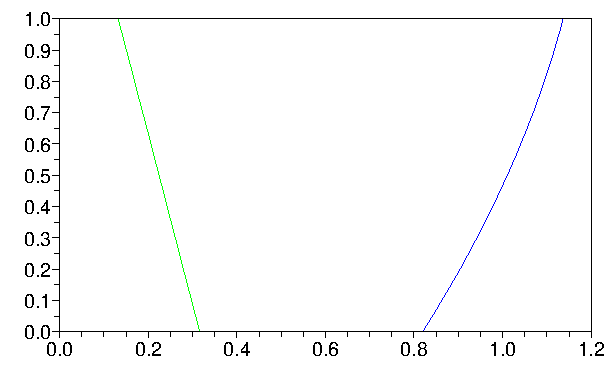
\includegraphics[width=0.8\linewidth]{vprofiles}\\[-2ex]
& $\ros(z) \eta/|\uu| \qtq{and} u(z)/\uu$\quad respectively
\end{tabular}
\caption{approximate vertical profiles at open channel flow equilibrium for which $g_x\eta/\uu^2=0.0031$\,.}
\label{fig:vp}
\end{figure}%
Figure~\ref{fig:vp} displays a sample of the vertical profile of the rate of strain~$\ros$ and of the lateral velocity~$u$. This equilibrium flow resolves the shear in the lateral velocity and the increase in rate of strain near the bed.  Our analysis does not attempt to resolve the turbulent log layer: we assume the details of dynamical interest are those determined by the relatively large scale of the fluid depth.

The set of such profiles in the vertical, and their nonlinear interactions, form a slow manifold.
The evolution on this slow manifold of the mean lateral velocities $\uu$~and~$\vv$ is dictated by turbulent bed drag limiting gravitational forcing:  ??
\begin{align}
\frac{d\uu}{dt}=& { 
-\frac{\sqrt2\,3c_t(1+c_u)}{(1+2c_u)(1+3c_u+3c_u^2)} }
\frac{\gamma \uu^2}\eta
+\frac{\rat34+3c_u+3c_u^2}{1+3c_u+3c_u^2}g_x
\nonumber\\&{}
+\Ord{\gamma^2+g_x^2+\partial_x}
\label{eq:gux}
\end{align}
Upon putting the artificial parameter $\gamma=1$ to recover the physical model, this evolution predicts an equilibrium channel flow at a mean velocity of
\begin{equation}
\uu=\frac12\left[ \frac{(1+2c_u)^3}
{\sqrt2c_t(1+c_u)} \right]^{1/2}\sqrt{g_x\eta} \,.
\end{equation}
For example, choosing $c_t=0.020$ and $c_u=1.848\approx 13/7\approx 11/6$ gives about the correct channel flow \emph{and} gives about the correct eddy viscosity when compared with observations of open channel flow~\cite[e.g.]{Nezu05}.



\subsection{Overview}

Denote free surface thickness~$\eta(x,y,t)$ by~\verb|h|, mean lateral velocities $\uu(x,y,t)$ and~$\vv(x,y,t)$ by \verb|uu|~and~\verb|vv|, and their
evolution $\eta_t=\verb|gh|$, $\uu_t=\verb|gu|$ and  $\vv_t=\verb|gv|$.  The Reynolds
number~\verb|re|, and the coefficients of lateral and normal
gravitational forcing are Gravity numbers \verb|grx|~and~\verb|grz|.  Construct an
asymptotic solution of the Smagorinski equations in terms of
$\eta$, $\uu$ and~$\vv$ to some order of nonlinearity in $\uu$~and~$\vv$ and some order
of lateral derivatives $\partial_x$~and~$\partial_y$.

Decide upon how the asymptotic expansions of the solution are to be
truncated.  Then iteratively update the velocity and pressure fields to
solve the Smagorinski equations and boundary conditions.  The
iteration continues until the governing equations are satisfied; that is, their
residuals are zero to the order of truncation.




\section{Preamble}

Improve printing by factoring with respect to these variables.  It is
a matter of taste and may be different depending upon what one wishes
to investigate in the algebraic expressions.

\begin{reduce}
on div; off allfac; on revpri; 
factor vv,uu,qq,rqq,h,ct,gx,gz,gam,r2;
\end{reduce}

\subsection{Define order parameters}

Use the operator \verb|h(m,n)| to denote lateral derivatives of the
fluid thickness,~$\partial_x^m\partial_y^n\eta$, and similarly \verb|uu(m,n)|~denotes
lateral derivatives of the mean shear,~$\partial_x^m\partial_y^n\uu$.  Also
define readable abbreviations for~$\eta$ and its first spatial
derivatives.  Note: use~\verb|d| to count the number of lateral
 derivatives so we can easily truncate the asymptotic expansion.

\begin{reduce}
operator h; operator uu; operator vv;
eta:=h(0,0); etax:=h(1,0)*d$ etay:=h(0,1)*d$
\end{reduce}

These operators must depend upon time and lateral space.  Then lateral
derivatives transform as $\partial_x\verb|h(m,n)|= \verb|h(m+1,n)|$\,, for
example.  Also, a time derivative transforms into lateral
derivatives of the corresponding evolution: for example,
$\partial_t\verb|h(m,n)|= \partial_x^m\partial_y^n\verb|gh|$\,.

\begin{reduce}
%preamble
depend h,xx,yy,tt; 
depend uu,xx,yy,tt; 
depend vv,xx,yy,tt; 
let { df(h(~m,~n),xx) => h(m+1,n)
    , df(h(~m,~n),yy) => h(m,n+1)
    , df(h(~m,~n),tt) => df(gh,xx,m,yy,n)
    , df(uu(~m,~n),xx) => uu(m+1,n)
    , df(uu(~m,~n),yy) => uu(m,n+1)
    , df(uu(~m,~n),tt) => df(gu,xx,m,yy,n)
    , df(vv(~m,~n),xx) => vv(m+1,n)
    , df(vv(~m,~n),yy) => vv(m,n+1)
    , df(vv(~m,~n),tt) => df(gv,xx,m,yy,n) 
    };
\end{reduce}


\subsection{Stretch the coordinates with the free surface}

Use stretched coordinates \verb|zz|, \verb|xx|, \verb|yy| and \verb|tt| to denote
$Z=z/\eta(x,t)$, $X=x$, $Y=y$ and $T=t$\,.  The free surface is then
simply $Z=1$\,.

\begin{reduce}
depend xx,x,y,z,t;
depend yy,x,y,z,t;
depend zz,x,y,z,t;
depend tt,x,y,z,t;
\end{reduce}

Then space-time derivatives transform according to 
\begin{displaymath}
    \D x{}=\D X{}-Z\frac{\eta_X}\eta\D Z{}\,,\quad
    \D y{}=\D X{}-Z\frac{\eta_Y}\eta\D Z{}\,,\quad
    \D t{}=\D T{}-Z\frac{\eta_T}\eta\D Z{}\,,\quad
    \D z{}=\frac1\eta\D Z{}\,.
\end{displaymath}
I neatly insert an automatic count of lateral $x$~derivatives
here, with~\verb|d|, in between $\partial_x$~and~$\partial_X$, and  in between $\partial_y$~and~$\partial_Y$.

\begin{reduce}
let { df(~a,x) => df(a,xx)*d-zz*etax/eta*df(a,zz)
    , df(~a,y) => df(a,yy)*d-zz*etay/eta*df(a,zz)
    , df(~a,t) => df(a,tt)-zz*gh/eta*df(a,zz)
    , df(~a,z) => df(a,zz)/eta
    };
\end{reduce}


\subsection{Operators used elsewhere}

For integrating in the vertical, use the linear operator~\verb|wsolv| as it is quicker than native integration.  This is the definite integral that is zero at the bed $\zs=0$\,.

\begin{reduce}
operator wsolv; linear wsolv;
let {wsolv(zz^~~n,zz) => zz^(n+1)/(n+1)
    ,wsolv(1,zz) => zz };
\end{reduce}

Similarly, it is quicker to use operators than to use the native integration to find the pressure.  This is the vertical integral (negative) that is zero at the surface $\zs=1$\,.

\begin{reduce}
operator psolv; linear psolv;
let {psolv(zz^~~n,zz) => (1-zz^(n+1))/(n+1)
    ,psolv(1,zz) => (1-zz) };
\end{reduce}

Variable \verb|qq| denotes the mean speed $\qq=\sqrt{U^2+V^2}$. Let \verb|rqq|~denotes its reciprocal.  The following transformation rules should be correct.  Either of the last two can be chosen.
\begin{reduce}
depend qq,uu(0,0),vv(0,0);
let { qq^2=>uu(0,0)^2+vv(0,0)^2
    , df(qq,~aa)=>(uu(0,0)*df(uu(0,0),aa)+vv(0,0)*df(vv(0,0),aa))*rqq
    };
depend rqq,qq;
let { df(rqq,~aa)=>-rqq^2*df(qq,aa)
    , rqq*qq=>1
    , qq^2=>(uu(0,0)^2+vv(0,0)^2)
    , vv(0,0)^2*rqq=>qq-uu(0,0)^2*rqq 
%    , uu(0,0)^2*rqq=>qq-vv(0,0)^2*rqq
    };
\end{reduce}

The linear operator \verb|usolv| solves $\partial_\zs^2 u'=\textsc{rhs}$
such that the bed boundary condition~\eqref{eq:bedbc} is always satisfied and that the mean of the solution~$u'$ is always zero to ensure $\uu$~remains the mean later velocity.

\begin{reduce}
operator usolv; linear usolv;
let { usolv(zz^~~n,zz) => (zz^(n+2) 
      -(cu+zz)/(n+3)/(cu+1/2) )/(n+2)/(n+1)
    , usolv(1,zz) => (zz^2 -(cu+zz)/3/(cu+1/2) )/2 };
\end{reduce}

Do not need it, but the linear operator \verb|mean| quickly computes the average of some field over the fluid thickness.

\begin{reduce}
operator mean; linear mean;
let { mean(zz^~~n,zz) => 1/(n+1)
    , mean(1,zz) => 1 };
\end{reduce}

I like to see how the iteration is proceeding.  For each equation, write out the number of terms in its residual throughout iteration.  Could also write out time since last length written.

\begin{reduce}
procedure mylength(res); 
begin 
%showtime; 
%return res;
return if res=0 then 0 else length(res);
end;
\end{reduce}




\section{Initialise with linear}

Start the iteration from the linear solution that the lateral velocity
$u=\uu (c_u+\zs)/(c_u+\rat12)$ and $v=??$ and all other fields are zero,
$w=p=0$\,.  The parameter~$c_u$ determines the turbulent slip on the bed and is to be determined to best fit experiment and/or observations.  The evolution of the `order parameters' is also zero:
$\uu_t=\verb|gu|=0$, $\vv_t=\verb|gv|=0$ and $\eta_t=\verb|gh|=0$\,.

\begin{reduce}
let r2^2=>2; % r2=sqrt2
u:=uu(0,0)*(cu+zz)/(cu+1/2); 
v:=vv(0,0)*(cu+zz)/(cu+1/2); 
p:=grz*(1-zz)*eta;
w:=gh:=gu:=gv:=0; 
\end{reduce}

Also set initial strains from the linear solution.

\begin{reduce}
exx:=df(u,x);
eyy:=df(v,y);
ezz:=df(w,z);
exz:=(df(u,z)+df(w,x))/2;
exy:=(df(u,y)+df(v,x))/2;
eyz:=(df(v,z)+df(w,y))/2;
\end{reduce}

Initially approximate the magnitude~$\ros$ of the strain-rate
tensor: the above iteration step assumes the strain rate 
is~$(\uu,\vv)\sqrt2/\eta/(1+2c_u)$ to leading approximation. 

\begin{reduce}
ros:=qq*r2/eta/(1+2*cu);
\end{reduce}

In the Smagorinski model \cite[e.g.]{Ozgokmen07} $c_t=(c_s\Delta/\eta)^2$ where arguments indicate $c_s\approx0.2$\,.   To match observations~\cite[e.g.]{Nezu05} of open channel flow equilibria we set $c_t=0.020$ from which the appropriate filter scale~$\Delta\approx 0.7 \eta $ consistent with significant mixing across the fluid layer as seen in Figures 14--15 by \cite{Janosi04}.  

\begin{reduce}
ct:=1/50; 
\end{reduce}

Set initial values for the stress.

\begin{reduce}
txx:=2*ct*eta^2*ros*exx;
tyy:=2*ct*eta^2*ros*eyy;
tzz:=2*ct*eta^2*ros*ezz;
txz:=2*ct*eta^2*ros*exz;
txy:=2*ct*eta^2*ros*exy;
tyz:=2*ct*eta^2*ros*eyz;
\end{reduce}

The bed slip-drag law requires coefficient.
\begin{reduce}
cu:=11/6;
\end{reduce}









\section{Truncate the asymptotic expansion}

There are lots of ways to truncate the asymptotic model.  The small
parameters available are:
\begin{itemize}
    \item  \verb|d| counting the number of $x$~derivatives of
    the slowly varying lateral spatial structure in any term;

    \item  the homotopy parameter~\verb|gam| varying between
    $\gamma=0$ for the artificial base problem and $\gamma=1$ for the
    physical fluid equations; and

    \item  \verb|grx|, \verb|gry| and~\verb|grz| being the lateral and normal
    components of gravity.
\end{itemize}
Note:  the velocity of the flow is not  small; consider the parameter~$\uu$ finite.

Usually we will make lateral gravity fairly small by scaling with the magnitude
of~$\partial_x$.

Initially omit all $x$~derivatives by setting $d=0$\,, later we
scale~$d$ with $\verb|eps|$ to get the relatively simple but interesting
model with errors~$\Ord{\gamma^{3/2}+g_x^{3/2}+g_z^3+\partial_x^3}$.\footnote{We need to check the algorithm at $\Ord{g_x^3}$.}  We need not make normal gravity~$g_z$ small as here, but doing so removes some messy terms.

\begin{reduce}
d:=eps;
grz:=eps*gz;
grx:=eps^2*gx;
gry:=0;
gamm:=eps*gam;
factor eps;
\end{reduce}

For now truncate to relatively low order,~$\Ord{\gamma^{3/2}+g_x^{3/2}+g_z^3+\partial_x^3}$, in spatial derivatives and boundary condition artifice (can do $\Ord{\epsilon^4}$ if no spatial variations):   

\begin{reduce}
let { eps^3=>0 };
\end{reduce}

\section{Invoke the iterative loop}
\begin{reduce}
for iter:=1:9 do begin ok:=1;
write "ITERATION ",iter;
\end{reduce}






\section{Update~$w$ with continuity and no flow through bed}

The nondimensional \pde{}s for the incompressible fluid flow include
the continuity equation
\begin{equation}
    \divv\vec q=\D xu+\D yv+\D zw=0\,,
\end{equation}
to be solved with no flow through the bed,
\begin{equation}
   w=0\quad\text{on}\quad z=0\,.
    \label{eq:nobed}
\end{equation}
As with all field variables in this model, the quantities $u$, $v$, $w$ and~$p$ are averaged over the ensemble of turbulent flows.
Compute the residual of the continuity equation, then update the
vertical velocity~$w$ by integrating from the bed, $\zs=0$\,.  The variable~\verb|ok| stores whether all residuals are so far zero in this iteration.

\begin{reduce}
resc:=df(u,x)+df(v,y)+df(w,z);
write length_resc:=mylength(resc);
ok:=if resc=0 then ok else 0;
w:=w+(dw:=-eta*wsolv(resc,zz));
\end{reduce}

The $\zs$ component of the stress and rate-of-strain tensor should be, and might need to be, updated from this correction to the normal velocity;  the magnitude of the rate-of-strain tensor is unaffected (to leading order).  But surely we do not have to do this here as it is computed again a little later??

\begin{reduce}
ezz:=ezz+df(dw,zz)/eta;
tzz:=tzz+2*r2*ct/(1+2*cu)*qq*df(dw,zz);
\end{reduce}





\section{Update the free surface evolution}

The kinematic condition at the free surface, 
\begin{equation}
    \D t\eta+u\D x\eta+v\D y\eta=w\quad\text{on}\quad z=\eta\,,
\end{equation}
gives the evolution of the fluid thickness~\verb|h|.  It dominantly arises from the normal velocity.

\begin{reduce}
gh:=sub(zz=1,w-u*etax-v*etay);
\end{reduce}










\section{Update pressure from vertical momentum and surface normal stress}

The nondimensional momentum equation is
\begin{equation}
    \D t{\vec q} +\vec q\cdot\grad\vec q
    =-\grad p +\divv\vec\tau +\vec{g}\,,
\end{equation}
where $\vec\tau$~is the
nondimensional deviatoric eddy stress tensor, and $\vec g$~is the direction of gravity; when the substrate slopes, $\vec{g}$~is not normal to the substrate. 
The vertical momentum equation is solved with the surface condition that
the turbulent mean, normal stress to the free surface is zero, that is, 
\begin{equation}
    -p+\frac{\tau_{zz} -2\eta_x\tau_{xz} -2\eta_y\tau_{yz}
    +\eta_x^2\tau_{xx} +2\eta_x\eta_y\tau_{xy}+\eta_y^2\tau_{yy}}
    {1+\eta_x^2+\eta_y^2}
     =0 \quad\text{on }
    z=\eta\,.
\end{equation}

Compute the residuals of the vertical momentum equation and the
zero normal stress on the free surface.  The recent change to the normal velocity affects the pressure update.

\begin{reduce}
resw:=df(w,t)+u*df(w,x)+v*df(w,y)+w*df(w,z) 
    +df(p,z) +grz -df(txz,x)-df(txy,y)-df(tzz,z);
write length_resw:=mylength(resw);
restn:= sub(zz=1,-p*(1+etax^2+etay^2) 
    +tzz -2*etax*txz -2*etay*tyz
    +etax^2*txx+2*etax*etay*txy+etay^2*tyy );
write length_restn:=mylength(restn);
ok:=if {resw,restn}={0,0} then ok else 0;
\end{reduce}

Update the pressure field~$p$ by integrating down from the free
surface $\zs=1$\,; we use the linear operator \verb|psolv| to solve
$\partial_\zs p'=-\textsc{rhs}$ such that $p'=0$ at
$\zs=1$\,.

\begin{reduce}
p:=p+eta*psolv(resw,zz)+restn;
\end{reduce}








\section{Update stress, $u$~and~$v$ from lateral momentum and surface tangential stress}




\subsection{Smagorinski large eddy stress-shear closure}

Now the strain-rate tensor
\begin{displaymath}
	\ros_{ij} =\frac12\left( \D{x_j}{u_i} +\D{x_i}{u_j}\right) \,.
\end{displaymath}

\begin{reduce}
exx:=df(u,x);
eyy:=df(v,y);
ezz:=df(w,z);
exz:=(df(u,z)+df(w,x))/2;
exy:=(df(u,y)+df(v,x))/2;
eyz:=(df(v,z)+df(w,y))/2;
\end{reduce}


Then the stress tensor for the fluid is $\sigma_{ij}=-p\delta_{ij}
+2\rho\nu \ros_{ij}$\,: when the viscosity~$\nu$ is constant this
models a Newtonian fluid; but here the Smagorinski closure for
turbulent flow  is that this eddy viscosity varies linearly with
strain-rate magnitude (analogous to a shear thickening non-Newtonian fluid).
Define the magnitude~$\verb|ros|=|\ros|$, the second invariant of
the strain-rate tensor, where 
\begin{equation}
    |\ros|^2=\sum_{i,j}\ros_{ij}^2\,.
    \label{eq:cons}
\end{equation}

\begin{reduce}
rese:=exx^2+ezz^2+eyy^2+2*exz^2+2*exy^2+2*eyz^2-ros^2;
write length_rese:=mylength(rese);
ok:=if rese=0 then ok else 0;
ros:=ros+rese*eta*(cu+1/2)/r2*rqq;
\end{reduce}


Approximate the eddy viscosity at any point in the fluid as
proportional to the local strain-rate magnitude, 
\begin{equation}
    \nu=c_t\eta^2\ros \,,
    \label{eq:nut}
\end{equation}
where $c_t$~is a dimensionless constant to be chosen to fit experiments and/or observations.  For whatever~$c_t$ is chosen, the deviatoric stress tensor is $\tau_{ij}=2\nu\ros_{ij}=2c_t\eta^2\ros\ros_{ij}$.

\begin{reduce}
txx:=2*ct*eta^2*ros*exx;
tyy:=2*ct*eta^2*ros*eyy;
tzz:=2*ct*eta^2*ros*ezz;
txz:=2*ct*eta^2*ros*exz;
txy:=2*ct*eta^2*ros*exy;
tyz:=2*ct*eta^2*ros*eyz;
\end{reduce}



\subsection{Compute residuals of lateral momentum}

There must be no turbulent mean, tangential stress at the free surface,
\begin{eqnarray}&&
    (1-\eta_x^2)\tau_{xz}+\eta_x(\tau_{zz}-\tau_{xx})-\eta_y(\tau_{xy}+\eta_x\tau_{yz})=0
    \quad\text{on } z=\eta\,.
    \label{bc:tt} \\&&
    (1-\eta_y^2)\tau_{yz}+\eta_y(\tau_{zz}-\tau_{yy})
    -\eta_x(\tau_{xy}+\eta_y\tau_{xz})=0
    \quad\text{on}\quad z=\eta\,.
    \label{bc:tty}
\end{eqnarray}
Also, put a slip law on the mean bed to provide bed drag: 
\begin{eqnarray}&&
    u=c_u\eta \D zu \quad\text{on }z=0\,,
    \label{eq:bedbc}
    \\&&
    v=c_u\eta \D zv \quad\text{on }z=0\,,
    \label{eq:bedbcy}
\end{eqnarray}
for some constant~$c_u\approx 11/6$ to match open channel flow observations.  



To get centre manifold theory support for the slow manifold model of shallow water flow, modify the surface condition~(\ref{bc:tt}) on the tangential stress to have an artificial forcing proportional to the square of the local, free surface, velocity:
\begin{eqnarray}&&
    \left[
    (1-\eta_x^2)\tau_{xz}+\eta_x(\tau_{zz}-\tau_{xx})
    -\eta_y(\tau_{xy}+\eta_x\tau_{yz})
    \right] 
    \nonumber\\&&{}
    = \frac{(1-\gamma)\sqrt2c_t}{(1+c_u)(1+2c_u)} u\sqrt{u^2+v^2}
    \quad\text{on } z=\eta\,.
    \label{bc:tta}
    \\&&
    \left[
    (1-\eta_y^2)\tau_{yz}+\eta_y(\tau_{zz}-\tau_{yy})
    -\eta_x(\tau_{xy}+\eta_y\tau_{xz})
    \right] 
    \nonumber\\&&{}
    = \frac{(1-\gamma)\sqrt2c_t}{(1+c_u)(1+2c_u)} v\sqrt{u^2+v^2}
    \quad\text{on } z=\eta\,.
    \label{bc:ttay}
\end{eqnarray}
When we evaluate at $\gamma=1$ this artificial right-hand side becomes zero so the artificial surface condition~\eqref{bc:tta} reduces to the physical surface condition~\eqref{bc:tt}.  However, when both the parameter $\gamma=0$ and the lateral derivatives are negligible, $\partial_x=\partial_y=0$, then the lateral shear $u,v\propto c_u+\zs$ becomes a neutral mode of the dynamics.

The Euler parameter of a toy problem suggests introducing a factor $(1-\rat16\gamma)$ into the left-hand side of the tangential stress boundary condition~(\ref{bc:tta}) in order to improve convergence in the parameter~$\gamma$ when evaluated at the physically relevant $\gamma=1$\,.  This needs further exploration.  For the moment omit such a factor.

Compute the residuals of the lateral momentum equation, an artificial tangential stress on the free surface, and the bed boundary.  See that when $\gamma=0$ the free surface condition is effectively $\eta \partial_z u=u/(1+c_u)$\,, leading to our neutral mode $u\propto c_u+\zs$\,, namely $u=\uu(x,t)(c_u+\zs)/(c_u+\rat12)$\,; whereas when $\gamma=1$ the free surface condition reduces to zero tangential stress.

\begin{reduce}
resu:= df(u,t)+u*df(u,x)+v*df(u,y)+w*df(u,z) 
    +df(p,x) -grx -df(txx,x)-df(txy,y)-df(txz,z);
write length_resu:=mylength(resu);
resv:= df(v,t)+u*df(v,x)+v*df(v,y)+w*df(v,z) 
    +df(p,y) -gry -df(tyy,y)-df(txy,x)-df(tyz,z);
write length_resv:=mylength(resv);
resbu:=sub(zz=0,-u+cu*eta*df(u,z));
write length_resbu:=mylength(resbu);  
resbv:=sub(zz=0,-v+cu*eta*df(v,z));
write length_resbv:=mylength(resbv);  
ok:=if {resv,resu,resbu,resbv}={0,0,0,0} then ok else 0;
\end{reduce}



\subsection{Solve for updates to lateral velocity and rate-of-strain}

Update the lateral fields using an as yet unknown change in the evolution for the lateral mean velocities.  The lateral fields are coupled by the nonlinear stress-strain relation of the Smagorinski turbulent flow.

\begin{reduce}
u:=u+(du:=eta*(1+2*cu)*r2/(4*ct)*rqq^3*usolv(
    +(qq^2+vv(0,0)^2)*resu
    -uu(0,0)*vv(0,0)*resv ,zz));
v:=v+(dv:=eta*(1+2*cu)*r2/(4*ct)*rqq^3*usolv(
    +(qq^2+uu(0,0)^2)*resv
    -uu(0,0)*vv(0,0)*resu ,zz));
ros:=ros+(uu(0,0)*df(du,zz)+vv(0,0)*df(dv,zz))/(r2*eta)*rqq;
\end{reduce}



Now use the tangential stress on the free surface to determine the evolution corrections \verb|gud|~and~\verb|gvd|.  But first need to update part of the stress from changes in lateral velocity and rate-of-strain:  these updates to stress and strain are indeed needed to ensure that the residual of the lateral momentum equations are satisfied.  I would think that one extra iteration would do just as well, but upon testing find that it does not.

\begin{reduce}
exz:=(df(u,z)+df(w,x))/2;
eyz:=(df(v,z)+df(w,y))/2;
txz:=2*ct*eta^2*ros*exz;
tyz:=2*ct*eta^2*ros*eyz;
\end{reduce}

Then compute residuals of tangential stress equations.

\begin{reduce}
resttu:=(-sub(zz=1, 
    (1-0*gamm)*((1-etax^2)*txz+etax*(tzz-txx)-etay*(txy+etax*tyz))
    -(1-gamm)*r2*ct/(cu+1)/(2*cu+1)*u*qq) ); 
write length_resttu:=mylength(resttu);  
resttv:=(-sub(zz=1, 
    (1-0*gamm)*((1-etay^2)*tyz+etay*(tzz-tyy)-etax*(txy+etay*txz))
    -(1-gamm)*r2*ct/(cu+1)/(2*cu+1)*v*qq) ); 
write length_resttv:=mylength(resttv);  
ok:=if {resttu,resttv}={0,0} then ok else 0;
\end{reduce}


Update the lateral evolution based upon these residuals.
\begin{reduce}
gu:=gu-3*(1+2*cu)*(1+cu)
      /2/eta/(3+11*cu+12*cu^2)/(1+3*cu+3*cu^2)/(3+4*cu)
      *(((1+5*cu+8*cu^2)*uu(0,0)^2*rqq^2
      -(9+45*cu+80*cu^2+48*cu^3))*resttu
        +(1+5*cu+8*cu^2)*uu(0,0)*vv(0,0)*rqq^2*resttv);
gv:=gv-3*(1+2*cu)*(1+cu)
      /2/eta/(3+11*cu+12*cu^2)/(1+3*cu+3*cu^2)/(3+4*cu)
      *(((1+5*cu+8*cu^2)*vv(0,0)^2*rqq^2
      -(9+45*cu+80*cu^2+48*cu^3))*resttv
        +(1+5*cu+8*cu^2)*uu(0,0)*vv(0,0)*rqq^2*resttu);
\end{reduce}








\section{Postprocessing}

End the iterative loop.
\begin{reduce}
showtime;
if ok then write iter:=100000+iter;
end;
\end{reduce}

I may use these transformations to check on the dimensionality of various expressions.  But not at the moment.

\begin{verbatim}
dims:={ h(~m)=>nh*ll
    , uu(~m)=>mu*ll/tt
    , gx=>ngx*ll/tt^2 }$    
\end{verbatim}

Write out the final evolution on the slow manifold.

\begin{reduce}
r2:=sqrt(2)$ %eps:=1$
on rounded; print_precision 4;
write dhdt:=length(gh);
write dudt:=length(gu);  
write dvdt:=length(gv);  
\end{reduce}


Fin.\begin{reduce}end;\end{reduce}


\appendix
\section{Trace prints from sample execution}

\begin{verbatim}
d := eps

grz := gz*eps

             2
grx := gx*eps

gry := 0

gamm := gam*eps

ITERATION 1

length_resc := 7

length_resw := 76

length_restn := 3

length_rese := 51

length_resu := 92

length_resv := 87

length_resbu := 0

length_resbv := 0

length_resttu := 100

length_resttv := 101

Time: 320 ms

ITERATION 2

length_resc := 274

length_resw := 235

length_restn := 57

length_rese := 127

length_resu := 477

length_resv := 517

length_resbu := 0

length_resbv := 0

length_resttu := 74

length_resttv := 84

Time: 4370 ms

ITERATION 3

length_resc := 240

length_resw := 206

length_restn := 62

length_rese := 109

length_resu := 361

length_resv := 410

length_resbu := 0

length_resbv := 0

length_resttu := 74

length_resttv := 84

Time: 5610 ms  plus GC time: 10 ms

ITERATION 4

length_resc := 0

length_resw := 89

length_restn := 31

length_rese := 0

length_resu := 147

length_resv := 167

length_resbu := 0

length_resbv := 0

length_resttu := 0

length_resttv := 0

Time: 7290 ms  plus GC time: 20 ms

ITERATION 5

length_resc := 0

length_resw := 0

length_restn := 0

length_rese := 0

length_resu := 0

length_resv := 0

length_resbu := 0

length_resbv := 0

length_resttu := 0

length_resttv := 0

Time: 6990 ms  plus GC time: 10 ms

iter := 100005

dhdt := 4

dudt := 103

dvdt := 104
\end{verbatim}




\bibliographystyle{agsm}
\bibliography{ajr,bib}


\end{document}